\documentclass[12pt,a4paper]{article}

\usepackage[utf8]{inputenc}
\usepackage[english]{babel}
\usepackage{amsmath}
\usepackage{amsfonts}
\usepackage{amssymb}
\usepackage{graphicx}
\usepackage{cite}
\usepackage{hyperref}
\usepackage[left=2cm,right=2cm,top=2cm,bottom=2cm]{geometry}

\author{Communications Department}
\title{Communications. Physical Network Topology}


\begin{document}
\section{Aim of the document}
This document has been created in order to take a decision about the physical topology of our satellite's network and also to decide if we want or need global coverage or not. It is a very important decision due to the fact that reliability, performance and security are related with the physical topology. The most usual are: 
\begin{itemize}
\item Mesh
\item Star
\item Bus
\item Ring
\item Hybrid
\end{itemize}
In the following section the members of the groups will explain what they think the best option is, giving reasons for and against that decision. 
	% PROPUESTA BOYAN
	\section{Propuesta Boyan}
	\paragraph{}
	Options:
	\begin{itemize}
		\item Ideal case scenario: Global Coverage with lowest possible orbit.
	\item Not so ideal case scenario: Global Coverage with some satellites in a higher orbit acting as a hub.
	\end{itemize}
After reviewing \cite{Wood1998}, \cite{Muri2012}, \cite{Horne2002}, \cite{Wood2001}, \cite{BookchapterinServiceEfficientNetworkInterconnectionviaSatellite2002}, 
\cite{Goodwin1998}, \cite{Sun2015} and \cite{Baumann} my proposal is the next:
\newline

·Use of the \textbf{Manhattan Topology} for our constellation, mixed with a \textit{Walker Delta} or a \textit{Walker Polar} orbits configuration.
\\

%ISL can be very high, with  very high data rates and then, sat to ground can be lower but we can divide it through the network

\textit{"The Manhattan network is the underlying form of the ISL satellite constellation’s
network topology. This is a regular topology named after the regular grid street
pattern established in Manhattan Island, New York. It is a toroidal mesh network with
each node having four unidirectional links: two transmit and two receive
[Maxemchuk87], as shown in figure 2.9.
Manhattan networks have been extensively discussed in computing literature in the
context of parallel computing. The Manhattan network forms the basic topology of the
type (2) constellation. The Manhattan network is also known as a multiaccess mesh or
multimesh network [ToddHahne97]. The form of the Manhattan network with bidirectional
links is known as either the bi-directional Manhattan network, as the HR4-
net [ChungSharAg94], or as the shufflenet.
However, orbital geometry leads to differences from previously discussed Manhattan networks. In fact, the constellation network is a slightly variant form, with bidirectional
ISLs and with two half-twists where the sense of rotation changes due to
each satellite seeing its neighbours swap sides while ‘down’ remains constant as the
satellites reach and pass through their highest latitudes. The topologies of the space
segments of Iridium, Teledesic, and Spaceway NGSO can be considered as variations
on the type of bi-directional Manhattan network shown in figure 2.10."}\cite[p. 32]{Wood2001} \textbf{(en Mendeley)}

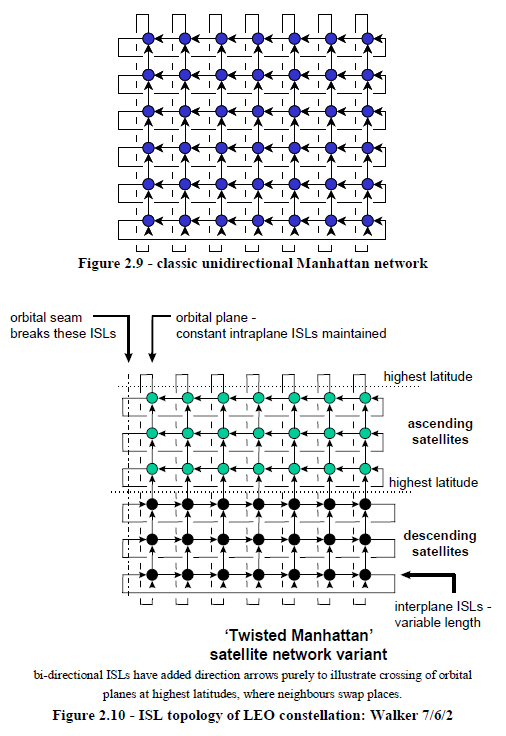
\includegraphics[scale=1]{parts/W_D}

	%Propuesta Eva 
	\section{Propuesta Eva}

	%Propuesta Josep
	\section{Propuesta Josep}
\subsection{Coverage}
I hold the view that we should offer as much coverage as possible, ideally full coverage, so that the range of clients is as broad as possible. So if it is technically feasible, I think we should intend to create a full coverage network. I agree with Eva, we do not need to create Ground Stations all around the world, it is responsability of the client, which is supposed to be a professional of the field, and therefore would have a proper Ground Station, hardware and knowledge to use and dominate it.
\subsection{Physical topology}
As it has been already said before, both mesh and star topology do not match our requirements. The option that Boyan has suggested (The Manhattan Topology) seems pretty nice, but Eva's suggestion too. In fact, they seem to be a bit similar. This seems a good direction to take. We should decide further details and maybe solve some little problems, but this is the kind of topology that I would take too. We should take into account the fact that distance between satellites might change, and be sure that in the furthest point, the communication is acceptable. We should also consider effects such as Doppler Effect (both the transmitter and the receiver are moving). This requires a further study, but this is the direction that I would definitely take. It would be nice if we could discuss it via Skype or any other communication programme, and decide exactly if Boyan's or Eva's option (though quite similar, a few differences exist).


	
	
	
	
	% BIBLIOGRAPHY
	\bibliography{boyan,eva}{}
	\bibliographystyle{plain}
	
	
\end{document}
